\chapter{Starless Openings}

\lettrine[lines=4]{\goudy W}{hen} we compare the stars of the first magnitude, which, on average, are certainly the nearest to us, with the nonnebulous telescopic stars, and further, when we compare the nebulous stars with unresolvable nebul\ae, for instance, with the nebula in Andromeda, or even with the so-called

\begin{wrapfigure}{r}{0.5\textwidth}
    \centering
    \fbox{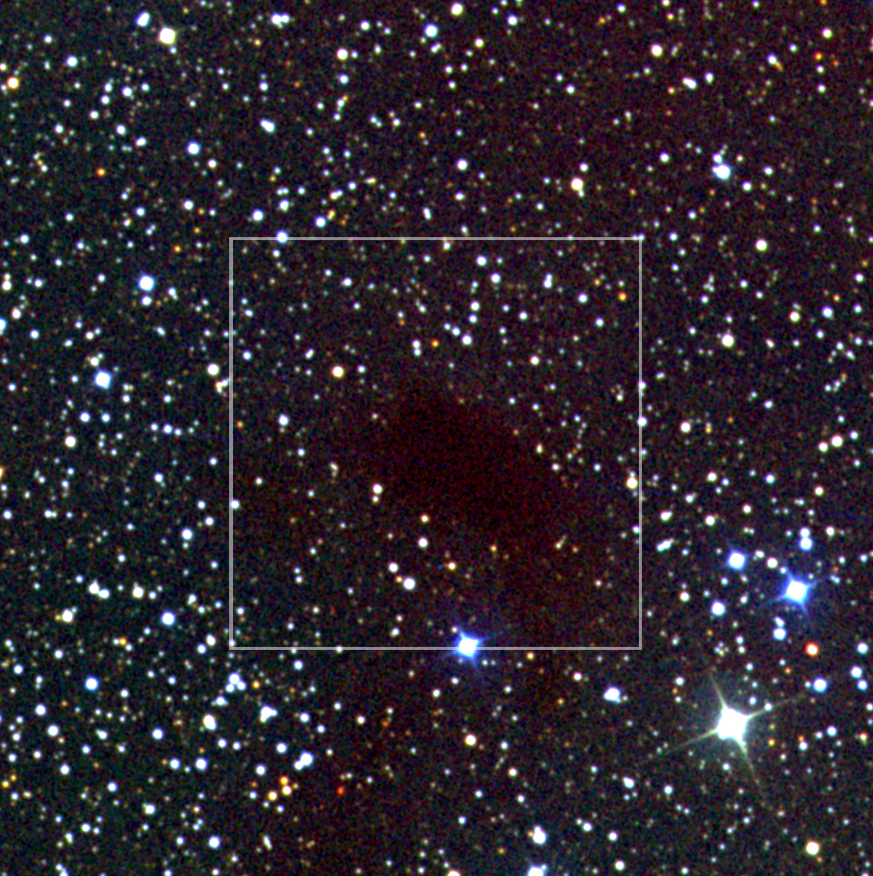
\includegraphics[width=0.5\textwidth]{../../pictures/_Starless__Core_L1014.jpg}}
    \caption{\footnotesize Starless Core L1014. Author: \href{https://commons.wikimedia.org/wiki/File:\%22Starless\%22_Core_L1014.jpg}{NASA}. Public domain.}
    \vspace{-10pt}
    \label{fig:starless-core}
\end{wrapfigure}

planetary nebulous vapor, a fact is made manifest to us by the consideration of the varying distances and the boundlessness of space, which shows the world of phenomena, and that which constitutes its causal reality, to be dependent upon the propagation of light. The velocity of this propagation is, according to Struve's most recent investigations, 166,072 geographical miles in a second, consequently almost a million times greater than the velocity of sound. According to the measurements of Maclear, Bessel, and Struve, of the parallaxes and distances of three fixed stars of very unequal magnitudes (a Centauri, 16 Cygni, and Lyre), a ray of light requires respectively 3, 93, and 12 years to reach us from these three bodies. In the short but memorable period between 1572 and 1604, from the time of Cornelius Gemma and Tycho Brahe to that of Kepler, three new stars suddenly appeared in Cassiopeia and Cygnus, and in the foot of Serpentarius. A similar phenomenon exhibited itself at intervals in 1670, in the constellation Vulpis. In recent times, even since 1837, Sir John Herschel has observed, at the Cape of Good Hope, the brilliant star 7 in Argo increase in splendor from the second to the first magnitude.\footnote{In December, 1837, Sir John Herschel saw the star 7 Argo, which till that time appeared as of the second magnitude, and liable to change, rapidly increase till it became of the first magnitude. In January, 1838, the intensity of its light was equal to that of Centauri. According to our latest information, Maclear, in March, 1843, found it as bright as Canopus; and even a Crucis looked faint by 7 Argo.} These events in the universe belong, however, with reference to their historical reality, to other periods of time than those in which the phenomena of light are first revealed to the inhabitants of the Earth. They reach us like the voices of the past. It has been truly said that with our large and powerful telescopic instruments we penetrate alike through the boundaries of time and space. We measure the former through the latter, for in the course of an hour a ray of light traverses over a space of 592 million miles. While, according to the theogony of Hesiod, the dimensions of the universe were supposed to be expressed by the time occupied by bodies in falling to the ground (the brazen anvil was not more than nine days and nine nights in falling from heaven to earth), the elder Herschel was of the opinion\footnote{Hence it follows that the rays of light of the remotest nebul\ae must have been almost two million years on their way, and that consequently, so many years ago, this object must already have had an existence in the sidereal heaven, in order to send out those rays by which we now perceive it. William Herschel, in the Phil. Trans. for 1802, p. 498. John Herschel, Astroz., 590. Arago, in the Annuaire, 1842, p. 334, 359, and 382-385.} that light required almost two million years to pass to the Earth from the remotest luminous vapor reached by his forty-foot reflector. Much, therefore, has vanished long before it is rendered visible to us. Much that we see was once differently arranged from what it now appears. The aspect of the starry heavens presents us with the spectacle of that which is only apparently simultaneous, and however much we may endeavor, by the aid of optical instruments, to bring the mildly radiant vapor of nebulous masses or the faintly glimmering starry clusters nearer, and diminish the thousands of years interposed between us and them, that serve as a criterion of their distance, it still remains more than probable, from the knowledge we possess of the velocity of the transmission of luminous rays, that the light of remote heavenly bodies presents us with the most ancient perceptible evidence of the existence of matter. It is thus that the reflective mind of man is led from simple premises to rise to those exalted heights of nature, where, in the light-illumined realms of space, myriad of worlds are bursting into life like the grass of the night.\footnote{From my brother's beautiful sonnet "Freiheit und Gesetz." (Wilhelm von Humboldt, Gesammelte Werke, bd. iv., 8. 358, No. 25.)}